%!TEX TS-program = xelatex

\useoutertheme{infolines}

\usepackage{xetexko}
\usepackage{mathtools}
\usepackage{amsmath}
\usepackage{fontspec}
\usepackage{hyperref}
\usepackage{graphicx}
\usepackage{listings}
\usepackage{makeidx}
\usepackage{indentfirst}
\usepackage{standalone}


%\setmainfont {NanumMyeongjo}
\setsansfont {Noto Sans CJK KR}
\setmainfont {Noto Sans CJK KR}
\setmonofont[Scale=0.8]{DejaVu Sans Mono}

\lstdefinestyle{diff}{
  belowcaptionskip=1\baselineskip,
  breaklines=true,
  frame=L,
  xleftmargin=\parindent,
  showstringspaces=false,
  % Diffstart
  morecomment=[f][\color{gray}]{@@},
  % Diffincl
  morecomment=[f][\color{Green}]{+},
  % Diffrem
  morecomment=[f][\color{Red}]{-},
  basicstyle=\footnotesize\ttfamily,
}

\lstdefinestyle{customtxt}{
  belowcaptionskip=1\baselineskip,
  breaklines=true,
  frame=L,
  xleftmargin=\parindent,
  showstringspaces=false,
  basicstyle=\footnotesize\ttfamily,
}

\lstdefinestyle{customc}{
  belowcaptionskip=1\baselineskip,
  breaklines=true,
  frame=L,
  xleftmargin=\parindent,
  language=C,
  showstringspaces=false,
  basicstyle=\footnotesize\ttfamily,
  keywordstyle=\bfseries\color{green!40!black},
  commentstyle=\itshape\color{purple!40!black},
  identifierstyle=\color{blue},
  stringstyle=\color{orange},
}


\hypersetup {
  colorlinks, linkcolor=blue
}

\title {Hideroot}
\author {perillamint}


\AtBeginSection[]
{
  \begin{frame}
    \frametitle{Index}
    \tableofcontents[currentsection]
  \end{frame}
}

\begin {document}

\begin{frame}
  \titlepage
\end{frame}

\section[Section]{루팅?}
\begin{frame}
  \frametitle{0x00. 루팅?}
  \framesubtitle{https://g.co/ABH}

  \begin{center}
    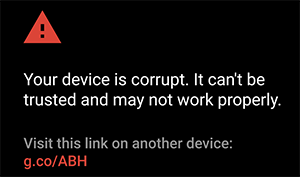
\includegraphics [width=100mm]{img/corrupted_nexus.png}
  \end{center}
\end{frame}

\begin{frame}
  \frametitle{0x00. 루팅?}
  \framesubtitle{https://g.co/ABH}

  \begin{itemize}
  \item 안드로이드 기기의 UID=0 권한을 가질 수 있게 도와주는 root helper 를 설치하는 행위
  \item<2-> 이를 통해, 앱이 원래대로라면 가질 수 없는 UID=0 권한을 획득할 수 있음
  \item<3-> 하지만 잠재적인 보안 이슈를 이유로, 많은 금융 앱들이 루트된 기기에서 동작을 거부함
  \item<4-> \textbf{이를 동작 가능하게 해 보자}
  \end{itemize}
\end{frame}
 
\section[Section]{루팅 탐지와 무력화}
\begin{frame}
  \frametitle{0x01. 루팅 탐지}
  \framesubtitle{libNSaferJNI.so}

  \begin{itemize}
  \item 1세대: 실행 후 에러 코드 체크
  \item <2-> 2세대: /system/xbin/su 유무 체크 (I wonder why they didn't used PATH envar)
  \item <3-> 3세대: NDK 에서 libc 함수들을 이용해 체크
  \item <4-> 4세대: system call 을 직접 호출해 체크 (iOS 에서 관찰됨)
  \end{itemize}
\end{frame}

\begin{frame}
  \frametitle{0x02. 루팅 탐지 무력화}
  \framesubtitle{Three Rings for the Elven-kings under the sky}

  \begin{itemize}
  \item 1세대: 가장 초보적 - 권한 허용 거부를 누른다.
  \item 2세대: XPosed 와 같은 Java hooking library
  \item 3세대: Cydia substrate (for NDK hook)
  \item 4세대: LKM rootkit, kernel patching, etc.
  \item <2-> 혹은 가장 귀찮은 방법: 앱을 패치해서 탐지 루틴을 무력화한다.
  \end{itemize}
\end{frame}

\section[Section]{Rootkit}
\begin{frame}
  \frametitle{0x03. User-mode rootkit - Xposed framework}
  \framesubtitle{Seven for the Dwarf-lords in their halls of stone}

  \begin{itemize}
  \item <1-> 일반 앱들에게, DalvikVM(or ART) 에 코드를 인젝션 할 수 있는 권한을 주는 프레임워크
  \item <2-> 이를 이용, Java 리플렉션을 통해 다른 앱 (특히 시스템 프레임워크) 에 코드를 주입, 기능 추가를 할 수 있음
  \item <3-> 은행 앱에 훅을 주입한다면?
  \item <4-> \textbf{2세대 루팅 탐지 우회 가능}
  \item <5-> 구현체: Rootcloak (Android)
  \end{itemize}
\end{frame}

\begin{frame}
  \frametitle{0x04. User-mode rootkit - Cydia Substrate}
  \framesubtitle{Nine for Mortal Men doomed to die}

  \begin{itemize}
  \item <1-> 네이티브 라이브러리 훅을 제공하는 프레임워크
  \item <2-> Apple iOS 의 Cydia Substrate 의 안드로이드 포트
  \item <3-> 이를 이용하면, NDK 의 libc 콜들을 후킹 가능
  \item <4-> 은행 앱이 부르는 libc 함수들을 후킹한다면?
  \item <5-> \textbf{3세대 탐지 우회 가능}
  \item <6-> 구현체: Rootcloak Plus (Android), kBankTweak (iOS)
  \end{itemize}
\end{frame}

\begin{frame}
  \frametitle{0x05. Kernel mode rootkit}
  \framesubtitle{One for the Dark Lord on his dark throne in the Land of Mordor}

  \begin{itemize}
  \item <1-> 직접적인 커널 변형.
  \item <2-> Ring 0 권한에서 실행
  \item <3-> 커널 내에서, 커널의 메모리 공간을 액세스하며, 이를 수정할 수 있음.
  \item <4-> 이를 이용한 system call 후킹을 통해, 유저랜드에 보여지는 것들을 조정할 수 있음.
  \item <5-> \textbf{일반적인} 앱들은 같은 권한을 가질 수 없음 -- 커널 코드 인젝션을 위해서는 루트 권한 필요
  \item <6-> 인-커널 코드가 자신을 Ring-3 어플리케이션으로부터 숨기고자 하면, 효과적으로 자기 자신을 숨길 수 있음.
  \item <7-> \textbf{4세대 탐지 우회 가능}
  \item <8-> 구현체: Hideroot PoC (Android (Linux kernel)), HideJB (iOS)
  \end{itemize}
\end{frame}

\section[Section]{LKM 루트킷 작성}
\begin{frame}
  \frametitle{0x06. 메모리 보호}
  \framesubtitle{Kernel panic - not syncing.}

  \begin{itemize}
  \item <1-> MMU 는 단순히 가상 메모리 주소를 실제 메모리 주소로 번역하는 것 이외에도 메모리 권한 관리를 한다.
  \item <2-> sys\_call\_table 을 변조하거나, 함수 프롤로그를 패치하기 위해서는 경우에 따라, 메모리 권한 변경이 필요할 수 있다.
  \item <3-> 몇몇 제조사 커널은, 이를 위한 함수를 제공하지만 (mem\_text\_address\_writable), 바닐라 커널에는 이가 존재하지 않는다
  \item <4-> 이에, 아키텍쳐별로, MMU 를 조작하기 위한 코드가 필요하다.
  \end{itemize}
\end{frame}

\begin{frame}
  \frametitle{0x07. 멀티-레벨 페이징}
  \framesubtitle{Walk through tables}

  \begin{itemize}
  \item <1-> MMU 는 메모리를 효율적으로(적은 메모리를 이용하여) 관리하기 위해, 다단계 페이징을 사용한다
  \item <2-> Qualcomm Snapdragon 800 의 경우 3단계 페이징이 사용된다.
  \item <3-> 페이지의 속성을 변경하기 위해서는, pgd $\rightarrow$ pud $\rightarrow$ pmd 순으로, 페이지 테이블을 찾아간 뒤
  \item <4-> PMD\_SECT\_APX 플래그를 지워주면 된다.
  \end{itemize}
\end{frame}

\begin{frame}
  \frametitle{0x08. 시스템 콜 후킹 - sys\_call\_table}
  \framesubtitle{}

  \begin{itemize}
  \item <1-> 시스템 콜이 불리우면, 플랫폼 종속적인 부분을 거쳐, 최종적으로 sys\_call\_table 에 도착한다
  \item <2-> sys\_call\_table 에 들어있는 함수 포인터 주소를 조작하면, 시스템 콜이 불렸을 때, 원하는 함수를 실행하게 할 수 있다.
  \item <3-> sys\_call\_table 의 메모리 보호를 해제했다면, 이의 내용을 변경할 수 있다.
  \item <4-> 이를 이용해, 시스템 콜들을 후킹할 수 있다.
  \end{itemize}
\end{frame}

\begin{frame}
  \frametitle{0x08. 시스템 콜 후킹 - sys\_call\_table}
  \framesubtitle{}

  \begin{center}
    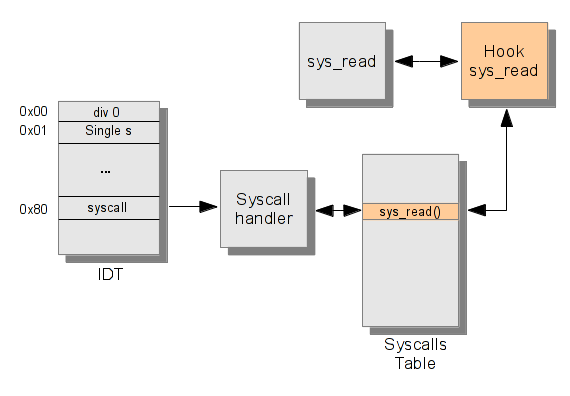
\includegraphics [width=100mm]{img/SSDT_hook_shellstorm_org.png}\cite{memorymanagement}
  \end{center}
\end{frame}

\begin{frame}
  \frametitle{0x09. 시스템 콜 후킹 - code hot patching}
  \framesubtitle{*Uptime* funk}

  \begin{itemize}
  \item <1-> 폰 노이만 구조 컴퓨터에서는, homoiconicity 가 성립한다.
  \item <1-> Code is data, data is code.
  \item <2-> 이에, 함수 프롤로그를 패치해서, 후킹 코드를 주입하면, 함수의 흐름을 돌릴 수 있다.
  \item <3-> 구현 사례: Ksplice (Oracle), kGraft (SUSE), kpatch (Red Hat), KProbes (Linux)
  \end{itemize}
\end{frame}

\begin{frame}
  \frametitle{0x09. 시스템 콜 후킹 - code hot patching}
  \framesubtitle{*Uptime* funk}

  \begin{center}
    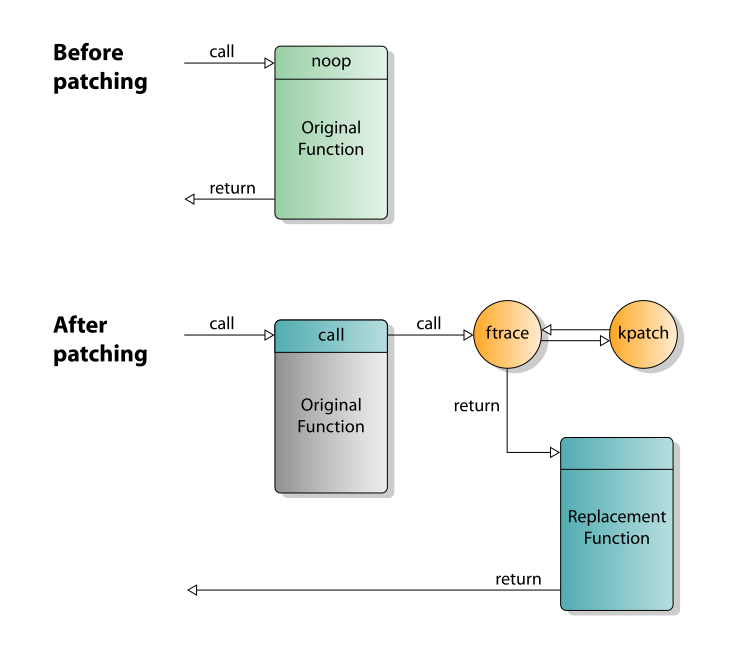
\includegraphics [width=80mm]{img/Linux_kernel_live_patching_kpatch.png}\cite{kpatch}
  \end{center}
\end{frame}

\begin{frame}
  \frametitle{0x0A. Code hot patching - in the wild}
  \framesubtitle{Non-ideal world}

  \begin{itemize}
  \item <1-> Kpatch나 MS Windows Hotfix 와 같은 솔루션은, 함수 프롤로그에 NOP sled 와 같은 여분 공간을 둠
  \item <2-> 하지만, Kpatch 미 대응 커널은, 핫패칭에 편리한 부분을 두지 않음.
  \item <3-> 이를 패치하기 위해서는, Detour 펑션을 활용해야 함
  \end{itemize}
\end{frame}

\begin{frame}
  \frametitle{0x0A. Code hot patching - in the wild}
  \framesubtitle{Non-ideal world}

  \begin{center}
    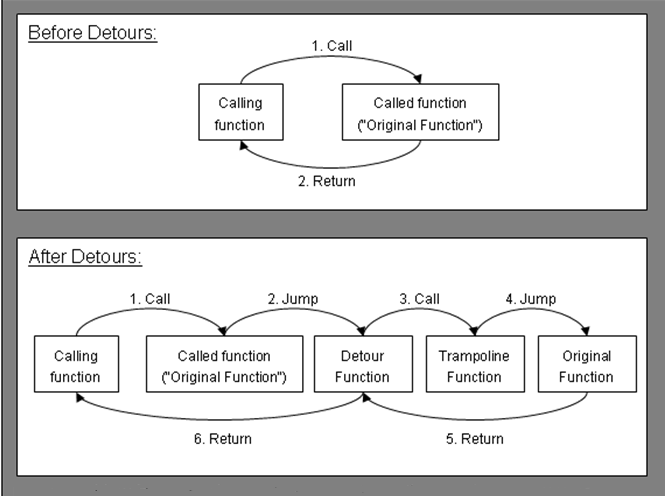
\includegraphics [width=80mm]{img/detour_nagareshwar_securityxploded_com.png}\cite{codeinject}
  \end{center}
\end{frame}

\begin{frame}
  \frametitle{0x0B. Code hot patching - CPU cache}
  \framesubtitle{}

  \begin{itemize}
  \item <1-> 코드 핫 패칭을 할 시에는, 코드를 수정 후, dcache 와 icache 를 동기화시켜주는 작업이 필요하다.
  \item <2-> 이를 위해서는, Level of Unification 까지 캐시를 flush 해, 모든 코어가 패치된 메모리를 같이 공유할 수 있도록 해야 한다.
  \item <3-> ARM infocenter 에서 찾을 수 있던 어셈 코드\cite{cp15c7,cache}로 테스트 했을 시
  \item <4-> Exynos 4412 에서는 잘 동작했지만, Snapdragon 800 에서는 동작하지 않았음
  \item <5-> 이를 해결하기 위한 작업이 필요하다. (May require NDA'ed Snapdragon datasheet)
  \end{itemize}
\end{frame}

\section[Section]{은닉 코드 구현}
\begin{frame}
  \frametitle{0x0C. 파일 은닉}
  \framesubtitle{Nazgûl}

  \begin{itemize}
  \item <1-> open(2), stat64(2), access(2), getdents64(2) 와 같은 시스템 콜을 후킹하면, 원하는 파일을 은닉할 수 있다.
  \item <2-> 이를 이용, Superuser.apk, /system/xbin/su 등을 특정 UID 에게만 숨기고, 나머지에는 노출한다면?
  \item <3-> $\rightarrow$ 루팅 탐지 우회 가능
  \end{itemize}
\end{frame}

\begin{frame}
  \frametitle{0x0C. 파일 은닉}
  \framesubtitle{Nazgûl}

  \begin{itemize}
  \item <1-> 안드로이드의 앱은 서로 다른 UID 를 갖는다
  \item <2-> \textbf{$\rightarrow$ 커널 세계에서, UID 를 이용해 앱을 구별하자!}
  \end{itemize}
\end{frame}

\begin{frame}
  \frametitle{0x0C. 파일 은닉}
  \framesubtitle{Nazgûl}

  \lstinputlisting [style=customc]{uid_check.c}
\end{frame}

\begin{frame}
  \frametitle{0x0C. 파일 은닉}
  \framesubtitle{Nazgûl}

  \lstinputlisting [style=customc]{my_sys_access.c}
\end{frame}

\begin{frame}
  \frametitle{0x0D. TBDs}
  \framesubtitle{//TODO: Do this}

  \begin{itemize}
  \item mmuhack.c 의 AMD64, AArch64 로의 포팅
  \item Qualcomm Snapdragon 이외의 다른 프로세서 (ex. HiSilicon Kirin, AllWinner, Samsung Exynos, etc) 에서의 테스트
  \end{itemize}
\end{frame}

\section[Section]{시연}
\begin{frame}
  \frametitle{0x0E. 스크린샷}
  \framesubtitle{금감원이 이 짤을 싫어합니다.}

  \begin{center}
    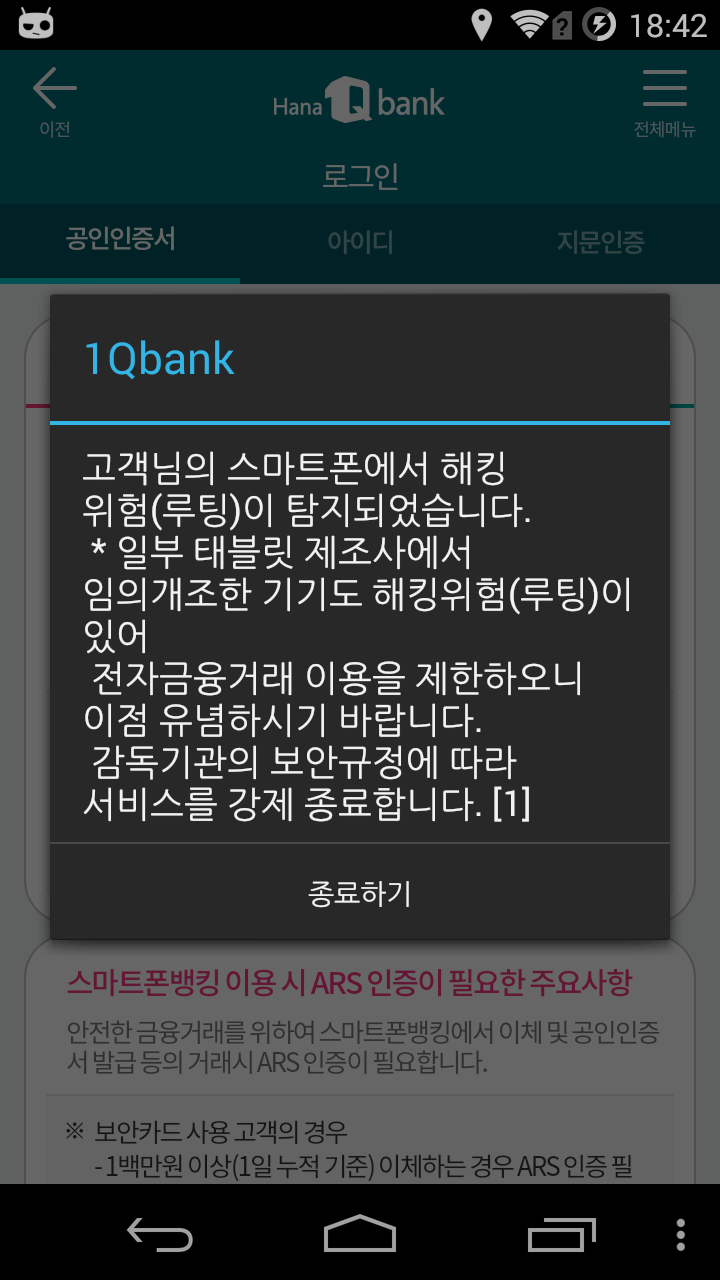
\includegraphics [width=40mm]{img/Hana1Qroot.png}
  \end{center}
\end{frame}

\begin{frame}
  \frametitle{0x0E. 스크린샷}
  \framesubtitle{금감원이 이 짤을 싫어합니다.}

  \begin{center}
    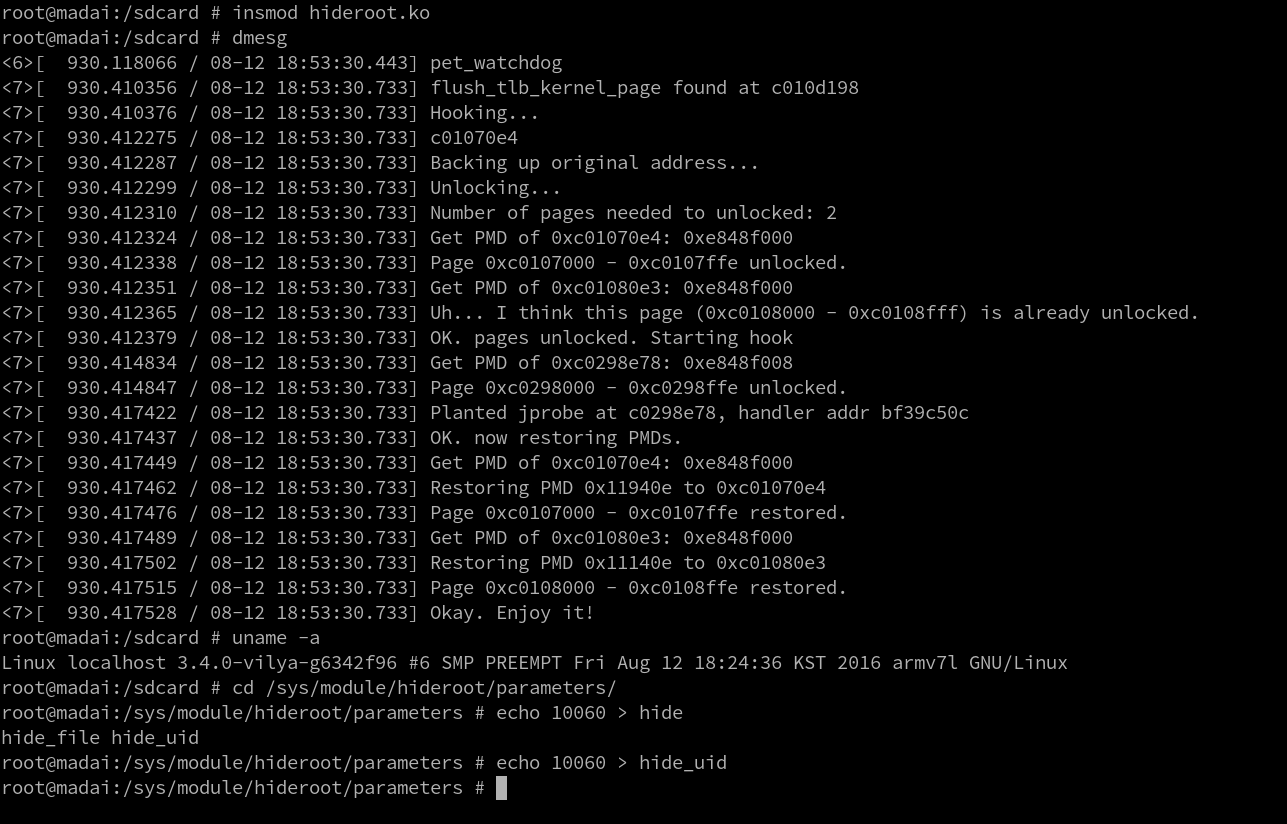
\includegraphics [width=100mm]{img/hideroot_init.png}
  \end{center}
\end{frame}

\begin{frame}
  \frametitle{0x0E. 스크린샷}
  \framesubtitle{금감원이 이 짤을 싫어합니다.}

  \begin{center}
    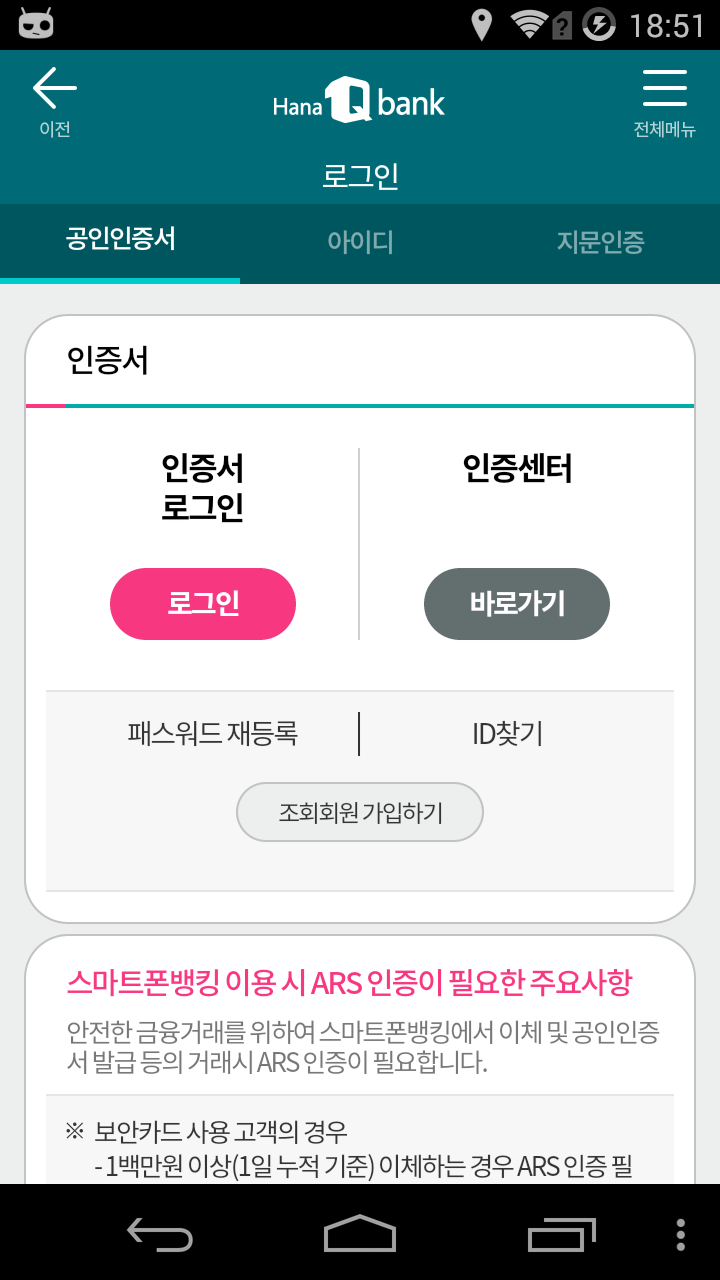
\includegraphics [width=40mm]{img/Hana1QrootBypass.png}
  \end{center}
\end{frame}

\begin{frame}
  \frametitle{0x0F. 시연}
  \framesubtitle{}

  \begin{center}
  This slide intentionally left blank
  \end{center}
\end{frame}

\begin{frame}
  \frametitle{0x10. GitHub repo}

  \url{https://github.com/perillamint/hideroot}\newline
  \begin{center}
    
\includegraphics [width=60mm]{img/ghrepo_qr.png}
  \end{center}
\end{frame}

\begin{frame}
  \frametitle{0x11. (su 바이너리 존재 유무보다) 진짜로 위험한 것들}
  \framesubtitle{\url{https://cve.mitre.org/}}

  \begin{itemize}
  \item <1-> 시장에 돌아다니는 EOL 장치들과 Outdated 장치들
  \item <2-> 취약한 장치를 노리는 One-day 익스플로잇들\cite{godless}
  \item <3-> 이러한 것들을 현재의 파일-기반 루팅 탐지가 검출해낼 수 있을까?
  \end{itemize}
\end{frame}

\section[Section]{끝}
\begin{frame}
  \frametitle{0x12. 끝}
  \framesubtitle{reboot(0xFEE1DEAD, 672274793, 0x4321FEDC);}

  \begin{center}
    Q \& A
  \end{center}
\end{frame}

\section[Section]{References}
\bibliographystyle {plain}
\bibliography {references}

\begin{frame}
  \frametitle{0x13. License}
  \framesubtitle{}
  Copyright (C)  2016 perillamint\linebreak
  Permission is granted to copy, distribute and/or modify this document
  under the terms of the GNU Free Documentation License, Version 1.3
  or any later version published by the Free Software Foundation;\linebreak
  with no Invariant Sections, no Front-Cover Texts, and no Back-Cover Texts.
  A copy of the license is included in the section entitled ``GNU
  Free Documentation License".
  \linebreak
  \linebreak
  %Repository address:\linebreak
  %\url{https://github.com/perillamint/K-HomeWRT-hack}
  \linebreak
  \linebreak
  
\includegraphics [width=30mm]{img/gfdl-logo-small.png}
\end{frame}

\end {document}
